\documentclass{beamer}
\usetheme{Frankfurt}
\usepackage{tabularx}
\usepackage{amsmath}


\renewcommand{\vec}{\mathbf}

\title{Analysis of Mathematical Optimization}
\subtitle{Some Classes, Problems, and Algorithms}
\author{by Liam Wrubleski}
\centering
\date{April 2020}
\begin{document}
	\maketitle
	\begin{frame}{Contents}
		\begin{itemize}
			\item Overview of Mathematical Optimization
			\item Linear Programming
			\begin{itemize}
				\item Simplex Algorithm
			\end{itemize}
			\item Mixed Integer Linear Programming
			\begin{itemize}
				\item Branch-and-Cut Simplex Algorithm
			\end{itemize}
			\item Convex Optimization
			\begin{itemize}
				\item Notable Subclasses
			\end{itemize}
			\item Non-Convex Optimization
			\begin{itemize}
				\item Wang et al. Stochastic Global Optimization
			\end{itemize}
		\end{itemize}
	\end{frame}
	
	% Overview
	\begin{frame}{Overview of Mathematical Optimization}
		\framesubtitle{General Overview}
		\begin{itemize}
			\item The general idea of mathematical optimization is to find an item $x$ in a set $D$ that minimizes the value of a function $f:D\to\mathbb{R}$.
		\end{itemize}
		\begin{block}{General Statement}
			Find \[m\in\mathbb{R}, x_0\in D\]
			such that\[m = f(x_0) = \min_{x\in D} \{f(x)\}\]
			for some set $D$, and \[f:D\to\mathbb{R}\]
		\end{block}
	\end{frame}

	\begin{frame}{Overview of Mathematical Optimization}
		\framesubtitle{Continuous Optimization \& Constraints}
		\begin{itemize}
			\item The function $f$ is referred to as the \textbf{objective function}.
			\item In general, the set $D$ may be any set, but here we only analyze sets $D\subseteq\mathbb{R}^n$, for any positive integer $n$ (this is called \textbf{continuous optimization}).
			\item Often, the set $D$ is specified using \textbf{constraint functions}:
			\begin{align*}
				D &= \{\vec{x}\in\mathbb{R}^n | g_i(\vec{x}) \leq 0, h_j(\vec{x}) = 0\}\\
				&g_i:\mathbb{R}^n\to\mathbb{R}, i=1,...,p\\
				&h_j:\mathbb{R}^n\to\mathbb{R}, j = 1,...,q
			\end{align*}
			\item The functions $g_i$ are \textbf{inequality constraints}, and $h_j$ are \textbf{equality constraints}.
		\end{itemize}
	\end{frame}
%
%	\begin{frame}{Overview of Mathematical Optimization}
%		\framesubtitle{Standard Form}
%		\begin{itemize}
%			\item In this case, we consider $f: \mathbb{R}^n\to\mathbb{R}$, as exploring potential solutions outside of $D$ allows for different solving methods.
%			\item When the problem is of the above form, it is generally expressed in \textbf{standard form}
%		\end{itemize}
%		\begin{block}{Standard form}
%			\begin{tabularx}{\textwidth}{l l l X}
%				minimize	& $f(\vec{x})$				&				& \\
%				subject to	& $g_i(\vec{x})\leq 0,$	& $i=1,...,p$	& \\
%				& $h_j(\vec{x}) = 0,$		& $j=1,...,q$	&
%			\end{tabularx}
%		\end{block}
%	\end{frame}
%
%	\begin{frame}{Overview of Mathematical Optimization}
%		\framesubtitle{Notes on Equivalence}
%		\begin{block}{Equality \& Inequality}
%			Any equality constraint may be expressed using two inequality constraints, using\[h_j(\vec{x})\leq 0, -h_j(\vec{x})\leq 0\]
%			Some optimization classes use only inequality constraints, but some take advantage of equality constraints to simplify computation.
%		\end{block}
%		\begin{block}{Maximization \& Minimization}
%			Problems attempting to maximize the value of $f(\vec{x})$ with some constraints can be computed by minimizing the value of $-f(\vec{x})$ subject to the same constraints, so maximize and minimize are effectively interchangeable.
%		\end{block}
%	\end{frame}
%
%	\begin{frame}{Linear Programming - LP}
%		\framesubtitle{Terminology}
%		\begin{block}{Programming}
%			Programming does not refer to computer programs. It was a term used by the US military to refer to proposed schedules, and made its way into mathematics via George B. Dantzig.
%		\end{block}
%		\begin{block}{Linear}
%			Linear in this context generally refers to affine in general mathematics. Linear programs are not themselves linear, but make use of the affine properties of their description.
%		\end{block}
%	\end{frame}

	\begin{frame}{Linear Programming - LP}
		\framesubtitle{Theory of Linear Programming}
		\begin{itemize}
			\item Linear Programming (LP) is a very simple class of mathematical optimization using only inequality constraints
			\item When expressed in standard form, a linear programming problem has the following properties
			\begin{align*}
				f(\vec{x}) &= c_1x_1 + c_2x_2 + ... + c_nx_n\\
				g_i(\vec{x}) &= a_{i1}x_1 + a_{i2}x_2 + ... + a_{in}x_n - b_i, i=1,...,m\\
				x_j &\geq 0
			\end{align*}
			\item This is usually expressed in standard form as 
		\end{itemize}
		\begin{tabularx}{\textwidth}{X l l X}
			& maximize		& $\vec{c}^T\vec{x}$		& \\
			& subject to	& $A\vec{x} \leq \vec{b}$	& \\
			& 				& $\vec{x} \geq \vec{0}$	& 
		\end{tabularx}
	\end{frame}
%
%	\begin{frame}{Linear Programming - LP}
%		\framesubtitle{Theory of Linear Programming}
%		\begin{itemize}
%			\item The objective function is linear, but the constraints are not. They are \textbf{affine}.
%		\end{itemize}
%		\begin{block}{Affine Functions}
%			We call a function $f:\mathbb{R}^n\to\mathbb{R}$ affine if and only if \begin{align*}
%				f(\vec{x}_1)=f(\vec{x}_2)=a\implies f(\alpha\vec{x}_1 + (1-\alpha)\vec{x}_2)=a,\\
%				\forall\alpha\in\mathbb{R}, \vec{x}_1,\vec{x}_2\in\mathbb{R}^n
%			\end{align*}
%		\end{block}
%	\begin{itemize}
%		\item Affine functions are more general than linear functions.
%	\end{itemize}
%	\end{frame}

	\begin{frame}{Linear Programming - LP}
		\framesubtitle{Theory of Linear Programming}
			\begin{itemize}
				\item The space of possible solutions satisfying all of the constraints may be considered an n-polytope.
				\item For $n=2, n=3$, this gives us an intuitive geometric interpretation, shown for two contrived examples in 2d and 3d respectively on the following slides.
				\item The blue polytope represents the space of possible solutions, the grey lines/planes represent the constraints, and the red arrow represents the direction of optimization.
			\end{itemize}
	\end{frame}	

%	\begin{frame}{Linear Programming - LP}
%		\framesubtitle{Theory of Linear Programming}
%		\begin{columns}[T]
%			\begin{column}{0.5\textwidth}
%				\small
%				\begin{tabularx}{\textwidth}{X l l X}
%					& maximize		& $x + 2y$		& \\
%					& subject to	& $-x-y+\frac{1}{\sqrt{2}}\leq 0$	& \\
%					& 				& $-x+y-\frac{\sqrt{2}+1}{\sqrt{2}}\leq 0$ & \\
%					& 				& $-x+y+\frac{\sqrt{2}+1}{\sqrt{2}}\leq 0$ & \\
%					& 				& $x-1-\sqrt{2}\leq 0$ & \\
%					& 				& $y-1-\sqrt{2}\leq 0$ & \\
%					&				& $x, y\geq 0$ &
%				\end{tabularx}
%			\end{column}
%			\begin{column}{0.5\textwidth}
%				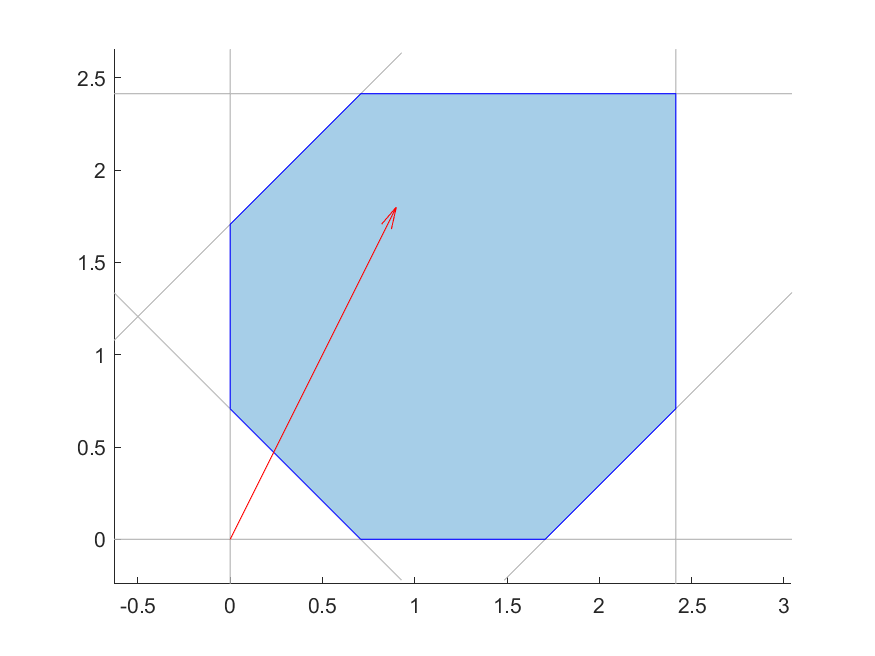
\includegraphics[width=\textwidth]{images/slides_ex1_2d.png}
%			\end{column}
%		\end{columns}
%	\end{frame}	
%
%	\begin{frame}{Linear Programming - LP}
%		\framesubtitle{Theory of Linear Programming}
%		\begin{columns}[T]
%			\begin{column}{0.5\textwidth}
%				\small
%				\begin{tabularx}{\textwidth}{X l l X}
%					& maximize		& $x + y + 3z$		& \\
%					& subject to	& $x+y+z-1\leq 0$	& \\
%					&				& $x, y, z\geq 0$ &
%				\end{tabularx}
%			\end{column}
%			\begin{column}{0.5\textwidth}
%				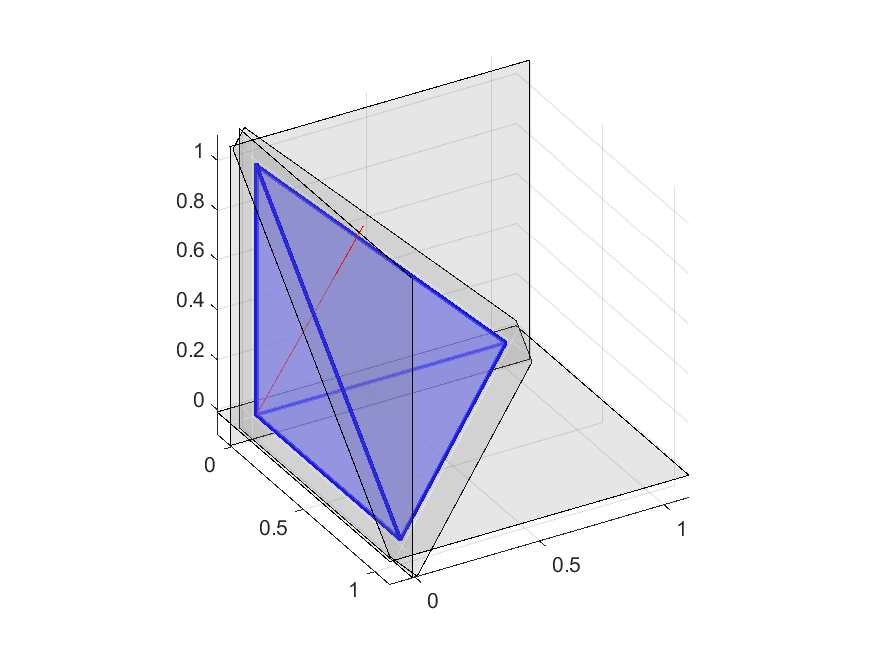
\includegraphics[width=\textwidth]{images/slides_ex2_3d.png}
%			\end{column}
%		\end{columns}
%	\end{frame}	

	\begin{frame}{Linear Programming - LP}
		\framesubtitle{Theory of Linear Programming}
		\begin{columns}[T]
			\begin{column}{0.5\textwidth}
				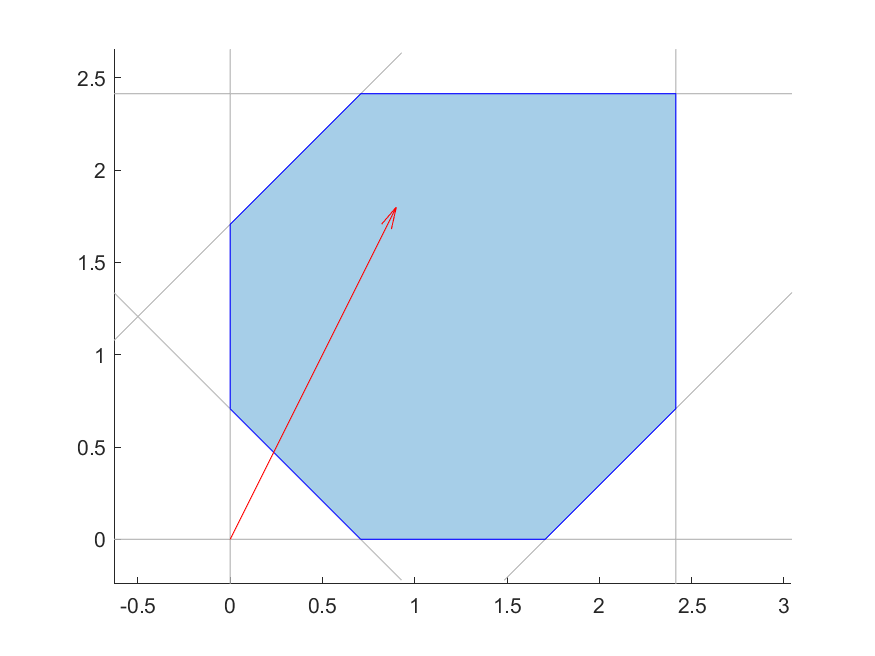
\includegraphics[width=\textwidth]{images/slides_ex1_2d.png}
				\small
				\begin{tabularx}{\textwidth}{X l l X}
					& maximize		& $x + 2y$		& \\
					& subject to	& $-x-y+\frac{1}{\sqrt{2}}\leq 0$	& \\
					& 				& $-x+y-\frac{\sqrt{2}+1}{\sqrt{2}}\leq 0$ & \\
					& 				& $-x+y+\frac{\sqrt{2}+1}{\sqrt{2}}\leq 0$ & \\
					& 				& $x-1-\sqrt{2}\leq 0$ & \\
					& 				& $y-1-\sqrt{2}\leq 0$ & \\
					&				& $x, y\geq 0$ &
				\end{tabularx}
			\end{column}
			\begin{column}{0.5\textwidth}
				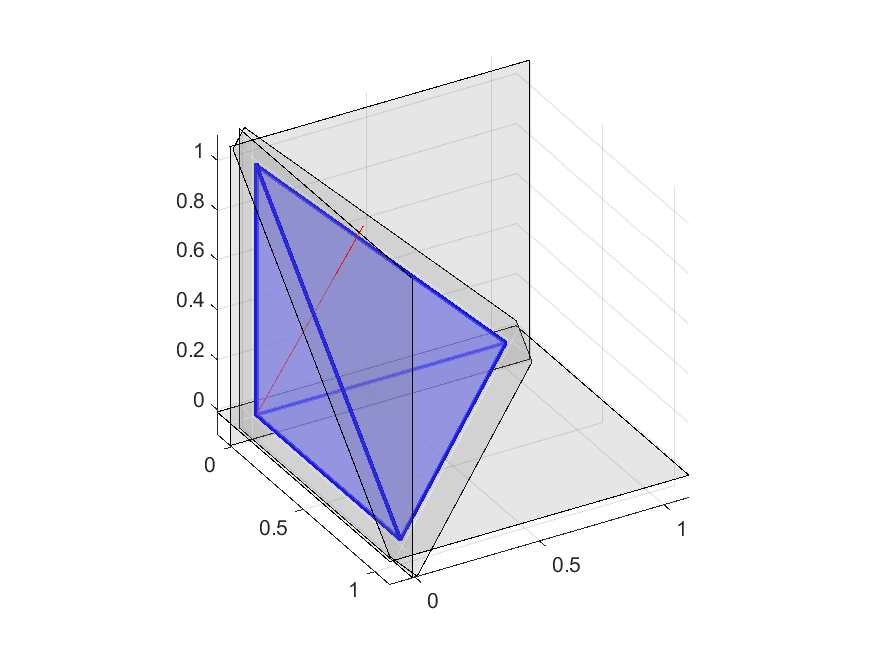
\includegraphics[width=\textwidth]{images/slides_ex2_3d.png}
				\small
				\begin{tabularx}{\textwidth}{X l l X}
					& maximize		& $x + y + 3z$		& \\
					& subject to	& $x+y+z-1\leq 0$	& \\
					&				& $x, y, z\geq 0$ &
				\end{tabularx}
			\end{column}
			
		\end{columns}
	\end{frame}

	\begin{frame}{Linear Programming - LP}
		\framesubtitle{Simplex Algorithm}
		\begin{itemize}
			\item Developed by George B. Dantzig in 1947 to solve LP problems, using the LP formulation of Leonid Kantorovich.
			\item Finds an optimal solution to an LP problem by moving along the edges of the polytope associated with the problem.
			\item Efficient on random problems, although inefficient in the worst case.
		\end{itemize}
	\end{frame}
%
%	\begin{frame}{Linear Programming - LP}
%		\framesubtitle{Simplex Algorithm}
%		\begin{itemize}
%			\item For each inequality $g_i(\vec{x})\leq 0$, a slack variable $s_i \geq 0$ is added to make an equality of the form $g_i(\vec{x}) + s_i = 0$.
%			\item The problem is then arranged into a matrix referred to as a \textbf{tableau}:\[
%			\begin{bmatrix}
%				1 & \vec{c}^T & \vec{0}_m^T & 0\\
%				\vec{0}_m & A & I_m & \vec{b}
%			\end{bmatrix}\]
%			where $I_m$ is the $m \times m$ identity matrix
%			\item We then move along the edges of the polytope for the original problem by performing operations called \textbf{pivots} on this tableau.
%		\end{itemize}
%	\end{frame}

	\begin{frame}{Linear Programming - LP}
		\framesubtitle{Simplex Algorithm}
		\begin{itemize}
			\item The exact operation of the algorithm takes too long to examine here, but will be examined in my paper.
			\item However, as a high level examination, each pivot moves along one edge of the polytope connected to the current point.
			\item This requires a number of row operations equal to the number of constraints in the model.
			\item We will examine the intermediate results of the algorithm for a small example.
		\end{itemize}
	\end{frame}

	\begin{frame}{Linear Programming - LP}
		\framesubtitle{Simplex Example}
		\begin{itemize}
			\item Suppose a farmer has 10 km$^2$ of land on which to grow wheat and barley, and that she has 17 kg of fertilizer and 13 kg of pesticide to use to grow it. 
			\item Every 1 km$^2$ of wheat requires 2 kg of fertilizer and 2 kg of pesticide, and sells for \$6000 of profit.
			\item Every 1 km$^2$ of barley requires 3 kg of fertilizer and 1 kg of pesticide, and sells for \$5000 of profit. 
			\item Suppose that the farmer needs to plant at least 1 km$^2$ of crops, regardless of any other consideration. 
		\end{itemize}
		How should the farmer plant her crops to maximize her profit?
	\end{frame}
%	
%	\begin{frame}{Linear Programming - LP}
%		\framesubtitle{Simplex Example}
%		\begin{itemize}
%			\item Let $x$ be the amount of land used for wheat, and $y$ be the amount of land used for barley.
%			\item Total 10 km$^2$ of land $\implies x + y\leq 10$.
%			\item Total 17 kg of fertilizer $\implies 2x + 3y\leq 17$.
%			\item Total 13 kg of pesticide $\implies 2x + y\leq 13$.
%			\item Plant at least 1 km$^2$ of land $\implies x + y \geq 1$.
%			\item Maximize profit (in thousands of dollars) $\implies \textrm{maximize } 6x + 5y$.
%		\end{itemize}
%	\end{frame}
%
	\begin{frame}{Linear Programming - LP}
		\framesubtitle{Simplex Example}
		\begin{tabularx}{\textwidth}{X l l X}
			& maximize		& $6x + 5y$		& \\
			& subject to	& $x + y - 10 \leq 0$	& \\
			& 				& $2x + 3y - 17 \leq 0$	& \\
			& 				& $2x + y - 13 \leq 0$ & \\
			& 				& $-x-y + 1 \leq 0$ & \\
			& 				& $x, y \geq 0$ & 
		\end{tabularx}
	\end{frame}
%
%	\begin{frame}{Linear Programming - LP}
%		\framesubtitle{Simplex Example}
%		\begin{columns}[T]
%			\begin{column}{0.2\textwidth}
%				\begin{align*}
%					x = 0\\
%					y = 0
%				\end{align*}
%				Note this point is not actually in the feasible space!
%			\end{column}
%			\begin{column}{0.8\textwidth}
%				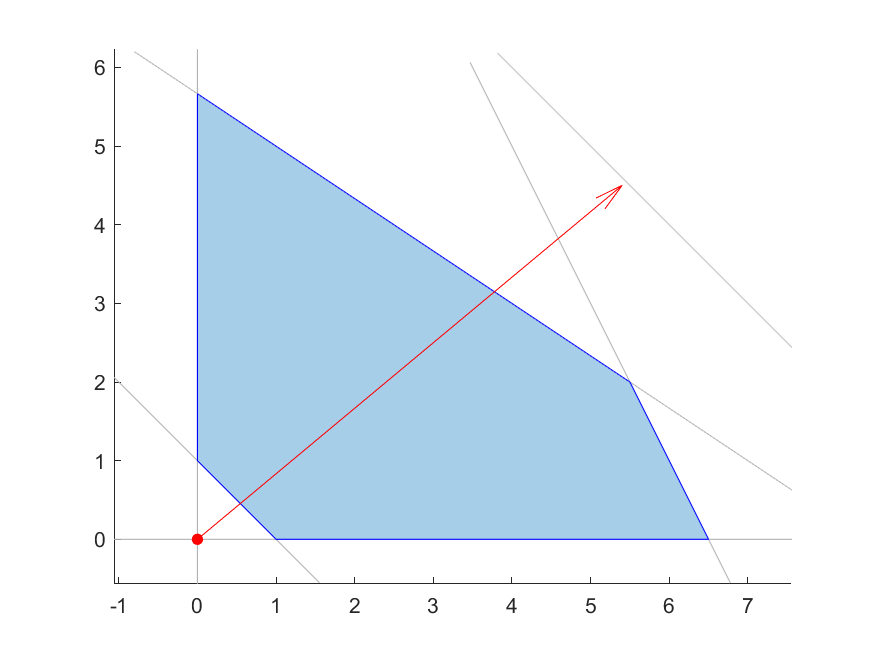
\includegraphics[width=\textwidth]{images/slides_ex3_simplex1.png}
%			\end{column}
%		\end{columns}
%	\end{frame}	
%
%	\begin{frame}{Linear Programming - LP}
%		\framesubtitle{Simplex Example}
%		\begin{columns}[T]
%			\begin{column}{0.2\textwidth}
%				\begin{align*}
%				x = 6.5\\
%				y = 0
%				\end{align*}
%			\end{column}
%			\begin{column}{0.8\textwidth}
%				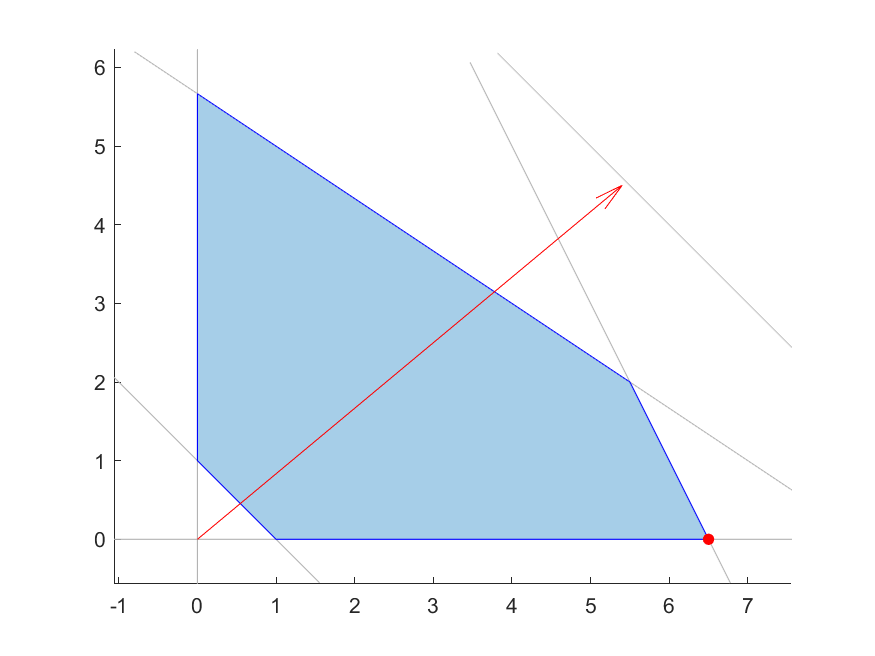
\includegraphics[width=\textwidth]{images/slides_ex3_simplex2.png}
%			\end{column}
%		\end{columns}
%	\end{frame}	

%\begin{frame}{Linear Programming - LP}
%	\framesubtitle{Simplex Example}
%	\begin{columns}[T]
%		\begin{column}{0.2\textwidth}
%			\begin{align*}
%			x = 5.5\\
%			y = 2
%			\end{align*}
%			This is our optimal point, with a maximized profit of \$43,000.
%		\end{column}
%		\begin{column}{0.8\textwidth}
%			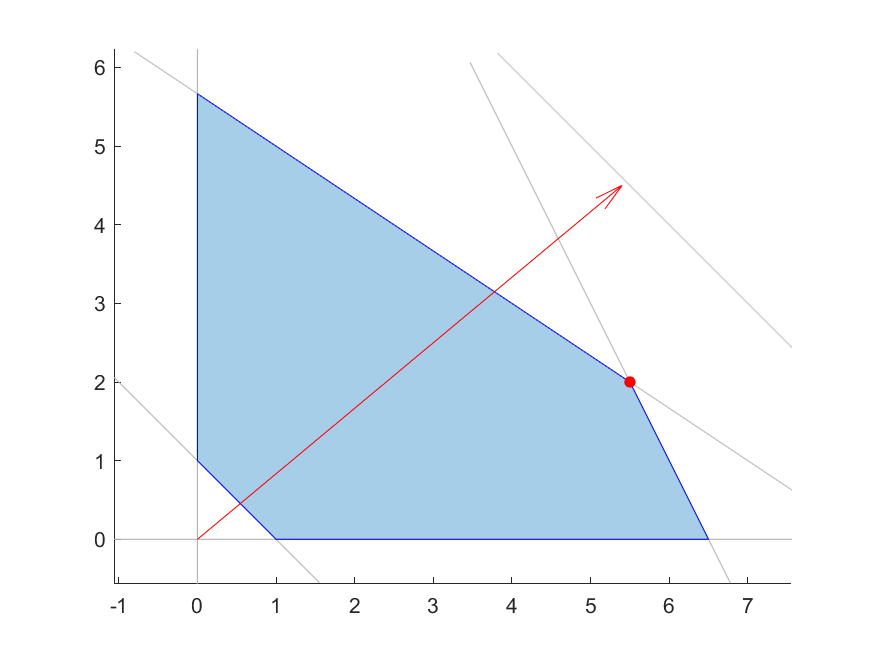
\includegraphics[width=\textwidth]{images/slides_ex3_simplex3.png}
%		\end{column}
%	\end{columns}
%\end{frame}	
	
	\begin{frame}{Linear Programming - LP}
		\framesubtitle{Simplex Example}
		\begin{columns}[T]
			\begin{column}{0.33\textwidth}
				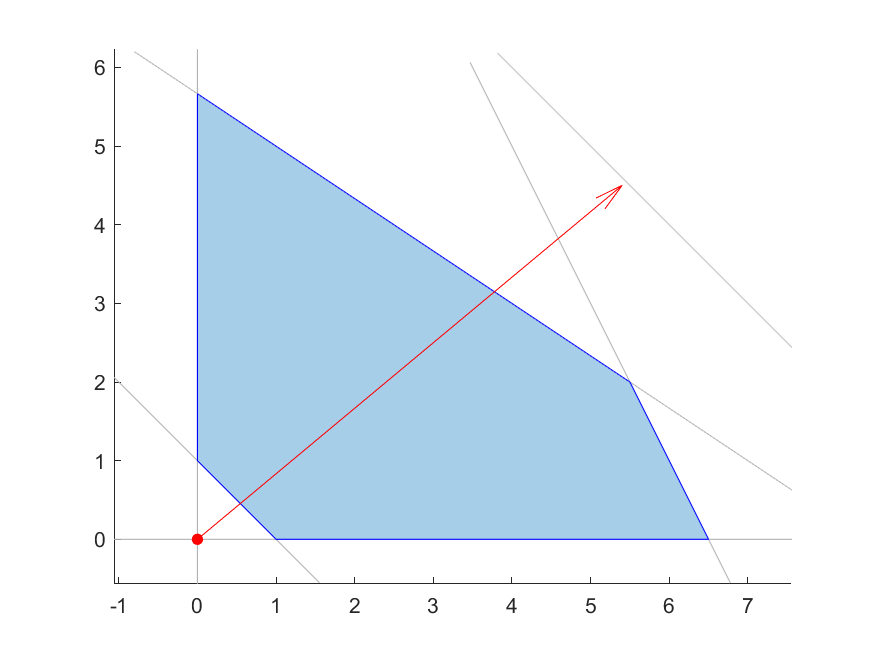
\includegraphics[width=\textwidth]{images/slides_ex3_simplex1.png}
				\begin{align*}
					x = 0\\
					y = 0
				\end{align*}
				Note this point is not actually in the feasible space!
			\end{column}
			\begin{column}{0.33\textwidth}
				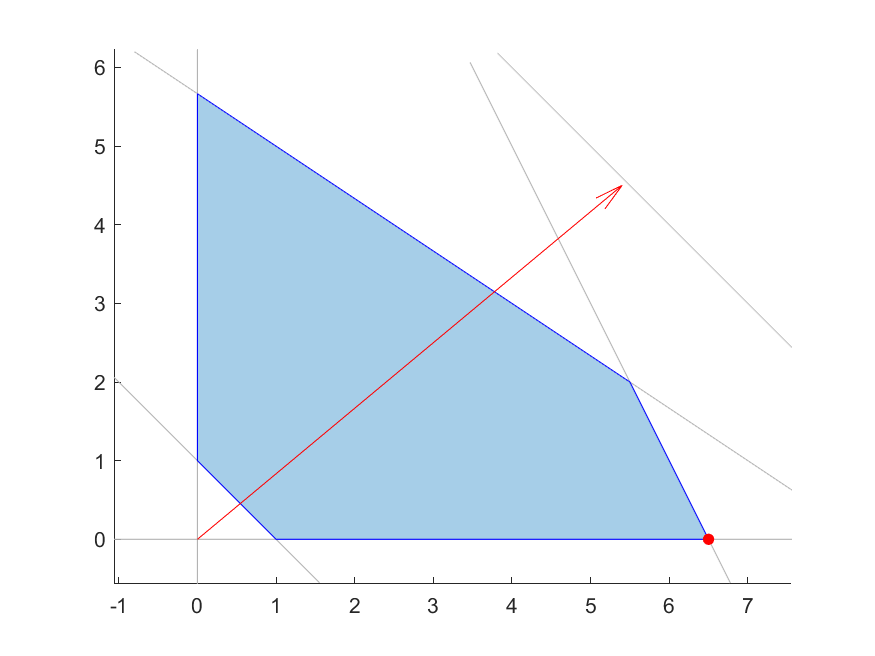
\includegraphics[width=\textwidth]{images/slides_ex3_simplex2.png}
				\begin{align*}
				x = 6.5\\
				y = 0
				\end{align*}
			\end{column}
			\begin{column}{0.34\textwidth}
				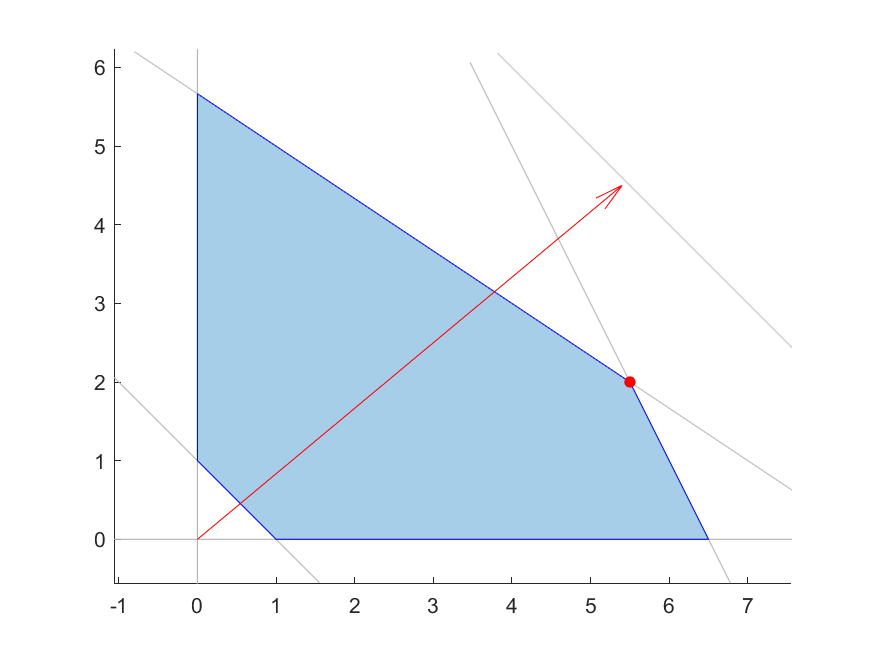
\includegraphics[width=\textwidth]{images/slides_ex3_simplex3.png}
				\begin{align*}
				x = 5.5\\
				y = 2
				\end{align*}
				This is our optimal point, with a maximized profit of \$43,000.
			\end{column}
		\end{columns}
	\end{frame}
%	
%	\begin{frame}{Linear Programming - LP}
%		\framesubtitle{Analysis}
%		\begin{itemize}
%			\item Each pivot requires $m-1$ row operations, and each row operation requires $n+m+2$ additions and $n+m+2$ multiplications.
%			\item When the algorithm is written with a good selection criterion for which edge to go along, it will not revisit any vertex of the polytope. However, as shown by Klee and Minty, there exist problems for which the algorithm will visit each vertex before terminating. 
%			\item This gives us that its worst case complexity is $O((nm + m^2)v)$, where $v$ is the number of vertices. However, as shown by Daniel Spielman, the average number of vertices visited is polynomial in the number of dimensions.
%		\end{itemize}
%	\end{frame}
%	
	\begin{frame}{Linear Programming - LP}
		\framesubtitle{Analysis}
		\begin{block}{Klee-Minty Cube}
			Klee and Minty showed that on the following problem, the usual simplex algorithm implementation visits every vertex of the polytope, giving a worst case complexity of $O(2^n)$.
			\begin{tabularx}{\textwidth}{X l l X}
				& maximize		& $\sum_{i=1}^{D}2^{D-i}x_i$		& \\
				& subject to	& $\sum_{i=1}^{k-1}2^{D-i+1}x_i + x_k+k\leq 5^k, k=1,...,D$	& \\
				& 				& $x_i \geq 0, i=1,...,D$
			\end{tabularx}
			The polytope for this problem looks like a squashed hypercube, which is where the name Klee-Minty Cube originates.
		\end{block}
	\end{frame}
	
	\begin{frame}{Mixed Integer Linear Programming - MILP}
		\framesubtitle{Theory}
		\begin{itemize}
			\item A variant of linear programming, with the additional requirement that some or all of the variables must have integer values. 
			\item This is a significantly more difficult variation of the problem.
		\end{itemize}
		\begin{block}{How much harder is it?}
			For reference, with just 120 variables, each of which can be either 0 or 1, computing all possibilities would take 16 times longer than the age of the universe on the world's fastest supercomputer, assuming each possibility takes only one floating point operation. Allowing each variable to also be 2, it would take a billion trillion times the age of the universe.
		\end{block}
	\end{frame}
%	
%	\begin{frame}{Mixed Integer Linear Programming - MILP}
%		\framesubtitle{Theory}
%		\begin{itemize}
%			\item The numbers in the previous slide may seem unreasonable, but many of the best known methods for solving these problems devolve to brute-force methodology. 
%			\item Further, although the examples up to now use very few variables, real-world problems often have hundreds of variables. For example, the standard method of assigning 40 people to 40 tasks uses at least 1600 integer variables.
%		\end{itemize}
%	\end{frame}
%	
	\begin{frame}{Mixed Integer Linear Programming - MILP}
		\framesubtitle{Theory}
		\begin{itemize}
			\item The way these problems are solved begins by solving the LP-relaxation of the problem.
		\end{itemize}
		\begin{block}{LP Relaxation}
			The LP-Relaxation of the MILP problem 
			\begin{tabularx}{\textwidth}{X l l X}
				& maximize		& $f(\vec{x})$		& \\
				& subject to	& $g_i(\vec{x}) \leq 0, i=1,...,m$	& \\
				& 				& $x_i \geq 0, i=1,...,n$ & \\
				& 				& $x_i\in\mathbb{Z}, i=1,...,k\leq n$ &
			\end{tabularx}
			is an LP problem with the same objective and inequality constraints, but without the integrality constraints.
		\end{block}
	\end{frame}

	\begin{frame}{Mixed Integer Linear Programming - MILP}
		\framesubtitle{Theory}
		\begin{itemize}
			\item Once the LP relaxation has been solved, it is used to find another solution to the constraints, but hopefully closer to a solution satisfying the integrality constraints. This is then repeated until it has been shown that the most recently found integer solution is optimal.
			\item The first common way of doing this is called \textbf{branch and bound}.
			\item The second common way of doing this is called \textbf{cutting planes}.
		\end{itemize}
	\end{frame}
%
%	\begin{frame}{Mixed Integer Linear Programming - MILP}
%		\framesubtitle{Branch and Bound}
%		\begin{itemize}
%			\item The value of the objective function for the solution to the LP relaxation is an upper bound for the value of the objective function for the MILP.
%			\item If any integral solution is found, the value of the objective function for that solution is a lower bound for the value of the objective function for the MILP.
%			\item If any integral solution is found with the value of the objective function equal to the upper bound, that solution is optimal.
%		\end{itemize}
%	\end{frame}
%
%	\begin{frame}{Mixed Integer Linear Programming - MILP}
%		\framesubtitle{Branch and Bound}
%		\begin{itemize}
%			\item Suppose the solution to the LP relaxation has some variables which are non-integer, but which have integrality constraints in the original MILP. Take $x_i$ to be one of these variables with value $x_i'$(the best methods for choosing which variable are generally trade-secrets, but many methods can be used). 
%			\item Create two new LP problems, one with the additional constraint $x_i \leq \lfloor x_i'\rfloor$, and the other with $x_i\geq \lceil x_i'\rceil$.
%			\item Solve each of these problems using branch and bound. If at any point the solution to the LP relaxation is worse than the current lower bound, prune that branch. If at any point the solution to the LP relaxation is integral, and is better than the current lower bound, update the lower bound.
%		\end{itemize}
%	\end{frame}
%	
%	\begin{frame}{Mixed Integer Linear Programming - MILP}
%		\framesubtitle{Cutting Planes}
%		\begin{itemize}
%			\item Given any non-integral solution, a cutting plane can be generated that removes the current solution, but no potential integral solutions.
%			\item While this is unlikely to produce a solution by itself, it decreases the upper bound of the MILP and potentially produces a better configuration for branching.
%		\end{itemize}
%	\end{frame}
%	
	\begin{frame}{Mixed Integer Linear Programming - MILP}
		\framesubtitle{Branch and Cut}
		\begin{itemize}
			\item This method combines branch-and-bound methods and cutting-plane methods to more quickly approach an integer value.
			\item Unfortunately, the best methods for balancing these techniques is an industry secret, and largely heuristic.
			\item In the worst case, branch-and-bound degenerates to brute force, and cutting planes generally do not help find integer solutions quickly, so even the best techniques are very difficult.
		\end{itemize}
	\end{frame}
%	
%	\begin{frame}{Mixed Integer Linear Programming - MILP}
%		\framesubtitle{Interesting Problems}
%		\begin{itemize}
%			\item Several well-known difficult problems can be expressed as MILP problems
%			\item The knapsack problem is very easily converted to a MILP.
%			\item The boolean satisfiability problem is also easily converted to a MILP. 
%			\item Many other NP-complete problems are also easily converted to MILP problems.
%			\item Real-world scheduling problems have a straightforward conversion to MILP problems. 
%		\end{itemize}
%	\end{frame}

	\begin{frame}{Mixed Integer Linear Programming - MILP}
		\framesubtitle{Problem Conversion}
		\begin{block}{Knapsack Problem}
			Consider $n$ items, each of which has a value $v_i$, a weight $w_i$, and a size $s_i$. You have a knapsack with a maximum weight $W$ and a maximum volume $S$. The knapsack problem is to determine which items should be placed in the knapsack to maximize the carried value. This can be expressed as a MILP as follows:
			\begin{tabularx}{\textwidth}{X l l X}
				& maximize		& $\vec{v}^T\vec{x}$	& \\
				& subject to	& $\vec{w}^T\vec{x} \leq W$	& \\
				& 				& $\vec{s}^T\vec{x} \leq S$ & \\
				& 				& $x_i\in\{0,1\}, i=1,...,n$ &
			\end{tabularx}
			Here, $x_i$ is 1 if you should pack item $i$, and 0 otherwise.
		\end{block}
	\end{frame}
%	
%	\begin{frame}{Mixed Integer Linear Programming - MILP}
%		\framesubtitle{Problem Conversion}
%		\begin{itemize}
%			\item The type of variable used in the above conversion is a \textbf{decision variable}. It's binary, and corresponds to making a decision (in this case, pack the item or not).
%			\item Not all integer constraints are decision variables. For example, if we had an arbitrary amount of each item in the above problem, we could have the variables correspond to how many of each item we pack.
%			\item These variables would still have an integrality constraint, as we generally assume we cannot pack part of an item.
%		\end{itemize}
%	\end{frame}
%	
	\begin{frame}{Convex Optimization}
		\framesubtitle{Theory}
		\begin{itemize}
			\item Linear programming is one of the simplest classes of convex optimization, and while it isn't convex, mixed-integer linear programming is often studied in the same areas.
			\item There are a lot of different kinds of convex optimization, but they all share some characteristics
			\begin{itemize}
				\item The objective function is convex, and
				\item The constraints are convex.
			\end{itemize}
		\end{itemize}
	\end{frame}

	\begin{frame}{Convex Optimization}
		\framesubtitle{Theory}
		\begin{block}{Convex Sets}
			A set $S$ is convex iff for any two points $a, b$, and any $\alpha\in[0,1]$, $\alpha a + (1-\alpha)b$ is also in the set $S$. Intuitively, if a line segment is drawn between the points $a$ and $b$, the line lies entirely within the set $S$.
		\end{block}
		\begin{block}{Epigraph}
			The epigraph of the function $f: \mathbb{R}^n\to\mathbb{R}$ is a set $S\subseteq\mathbb{R}^{n+1}$, with \[
				S = \{(x_0,x_1,...x_n) | x_0 \geq f(x_1,...x_n)\}
			\]
		\end{block}
		\begin{block}{Convex Functions}
			A function $f: \mathbb{R}^n\to\mathbb{R}$ is convex iff its epigraph is convex.
		\end{block}
	\end{frame}
%
%	\begin{frame}{Convex Optimization}
%		\framesubtitle{Theory}
%		\begin{itemize}
%			\item Convex optimization is simple relative to non-convex optimization, as if a local minimum of the objective function is found in the interior of the feasible space, then it is a global minimum.
%			\item If a local minimum is not found in the interior of the feasible space, then the minimum of the objective function on the feasible space is in the boundary of the feasible space (which is why strict inequalities are not used in LP).
%		\end{itemize}
%		\begin{block}{Note}
%			In LP and MILP, the sense is typically maximization. In convex optimization, the sense is typically minimization.
%		\end{block}
%	\end{frame}
%	
	\begin{frame}{Convex Optimization}
		\framesubtitle{Quadratic Programming - QP}
		\begin{itemize}
			\item Quadratic programming allows the objective function, but not the constraints functions, to take the form
			\[f(\vec{x}) = \vec{x}^TQ\vec{x} + \vec{c}^T\vec{x}\]
			\item One special case of quadratic programming is ordinary least squares, which will be explained shortly.
			\item Note that $Q$ must be positive semidefinite for $f$ to be convex.
		\end{itemize}
	\end{frame}
%
%	\begin{frame}{Convex Optimization}
%		\framesubtitle{Quadratic Programming - QP}
%		\begin{block}{Ordinary Least Squares}
%			Given $N$ test cases $\vec{x}_i\in\mathbb{R}^n, y_i\in\mathbb{R}$, find the constant vector $\vec{k}\in\mathbb{R}^n$ that minimizes the sum of the squared errors 
%			\begin{align*}
%			E &= \sum_{i=1}^{N}(\vec{k}^T\vec{x}_i - y_i)^2= \sum_{i=1}^{N}(\vec{k}^T\vec{x}_i\vec{x}_i^T\vec{k} - 2y_i\vec{x}_i^T\vec{k}+y_i^2)\\
%			&= \vec{k}^T(\sum_{i=1}^{N}\vec{x}_i^T\vec{x})\vec{k} + (\sum_{i=1}^{N}-y_i(2\vec{x}_i)^T)\vec{k} + \sum_{i=1}^{N}y_i^2\\
%			&= \vec{k}^TQ\vec{k} + \vec{c}^T\vec{k} + d
%			\end{align*}
%			As $d$ is a constant, any solution minimizing $E$ also minimizes $\vec{k}^TQ\vec{k}+\vec{c}^T\vec{k}$, and vice versa. This shows that ordinary least squares is an unconstrained quadratic programming problem.
%		\end{block}
%	\end{frame}
%	
	\begin{frame}{Convex Optimization}
		\framesubtitle{Quadratically Constrained Quadratic Programming - QCQP}
		\begin{itemize}
			\item A generalization of quadratic programming that allows the constraint functions to also take the form of convex quadratic functions, so the standard form looks like
			\begin{tabularx}{\textwidth}{X l l l X}
				& minimize		& $\vec{x}^TQ_0\vec{x} + \vec{p}_0^T\vec{x}$	& &\\
				& subject to	& $\vec{x}^TQ_i\vec{x} + \vec{p}_i^T\vec{x} + r_i \leq 0,$	& $i=1,...,m$ &\\
				&				& $A\vec{x} = \vec{b}$ & &
			\end{tabularx}
			where all $Q_i, i=0,...,m$ are positive semidefinite.
			\item Problems that can be formatted as QCQP problems come up often in statistics (for example, constraining the variance of a random variable)
		\end{itemize}
	\end{frame}
%
%	\begin{frame}{Convex Optimization}
%		\framesubtitle{Quadratically Constrained Quadratic Programming - QCQP}
%		\begin{block}{Portfolio optimization}
%			Suppose you are trying to invest in $n$ different stocks, represented by the random variable $\vec{p}\in\mathbb{R}^n$ with known mean $\bar{\vec{p}}$ and covariance $\Sigma$, where $p_i$ represents the price of stock $i$ at some point in the future divided by its price now. Let $x_i$ denote the amount you invest in stock $i$, and $B$ your total budget. Then your return is the random variable $\vec{p}^T\vec{x}$ with mean $\bar{\vec{p}}^T\vec{x}$ and variance $\vec{x}^T\Sigma\vec{x}$. Using the variance as a metric of risk, you might come up with this:
%			\begin{tabularx}{\textwidth}{X l l X}
%				& minimize		& $-\bar{\vec{p}}^T\vec{x}$	& \\
%				& subject to	& $\vec{x}^T\Sigma\vec{x} -\sigma_{max} \leq 0$	& \\
%				&				& $\vec{1}^T\vec{x} = B$ & 
%			\end{tabularx}
%			which maximizes your return, subject to a maximum allowable risk.
%		\end{block}
%	\end{frame}

	\begin{frame}{Convex Optimization}
		\framesubtitle{Second-Order Cone Programming - SOCP}
		\begin{itemize}
			\item A generalization of QCQP, this effectively allows the matrix $Q$ to have a single negative eigenvalue (making it no longer positive semidefinite. It's generally phrased, however, as follows
			\begin{tabularx}{\textwidth}{X l l l X}
				& minimize		& $\vec{f}^T\vec{x}$	& &\\
				& subject to	& $\lVert A_i\vec{x} + \vec{b}_i\rVert_2\leq\vec{c}_i^T\vec{x} + d_i,$	& $i=1,...,m$ &\\
				&				& $F\vec{x} = \vec{g}$ & &
			\end{tabularx}
			\item This kind of optimization is very useful in many real-world engineering problems, as the 2-norm can be used to constrain distances and placements of items. 
%			\item Squaring both sides of the inequality constraint $\lVert A\vec{x} + \vec{b}\rVert_2\leq\vec{c}^T\vec{x} + d$, we obtain
%			\begin{align*}
%				(A\vec{x}+\vec{b})^T(A\vec{x}+\vec{b}) &\leq (\vec{c}^T\vec{x} + d)^2\\
%				\vec{x}^T(A^TA)\vec{x} + 2\vec{b}^TA\vec{x} + \vec{b}^T\vec{b} &\leq \vec{x}^T\vec{c}\vec{c}^T\vec{x} + 2d\vec{c}^T\vec{x} + d^2
%			\end{align*}
%			so using the variables from QCQP, we have $Q=(A^TA-\vec{c}^T\vec{c}$, $p=2(\vec{b}^TA-d\vec{c}^T)$, and $r = (\vec{b}^T\vec{b}-d^2)$. 
		\end{itemize}
	\end{frame}
%	
%	\begin{frame}{Convex Optimization}
%		\framesubtitle{Geometric Programming - GP}
%		\begin{itemize}
%			\item Geometric programs have a slightly different standard form to other optimization problems
%			\begin{tabularx}{\textwidth}{X l l l X}
%				& minimize		& $f_0(\vec{x})$	& &\\
%				& subject to	& $f_i(\vec{x}) \leq 1,$	& $i=1,...,p$ &\\
%				&				& $g_i(\vec{x}) = 1,$ & $i=1,...,q$ &
%			\end{tabularx}
%			where $f_i(\vec{x})$ are \textbf{posynomials}, and $g_i(\vec{x})$ are \textbf{monomials}.
%		\end{itemize}
%		\begin{block}{Monomials \& Posynomials}
%			The word monomial has a different meaning in geometric programming from the rest of mathematics. Here, it means a function from $\mathbb{R}_{++}^n\to\mathbb{R}$, defined as $x\mapsto cx_1^{a_1}x_2^{a_2}...x_n^{a_n}$, with $c>0, a_i\in\mathbb{R}$.\\
%			A posynomial is any sum of this type of monomials.
%		\end{block}
%	\end{frame}
%	
%	\begin{frame}{Convex Optimization}
%		\framesubtitle{Geometric Programming - GP}
%		\begin{itemize}
%			\item GP problems are not generally convex, but all GP problems can be transformed into an equivalent convex optimization problem. By taking $y_i=\log(x_i), \tilde{f}_i(\vec{y})=\log(f_i(\exp{\vec{y}})), \tilde{g}_i(\vec{y})=\log(g_i(\exp{\vec{y}}))$, we end up with a convex optimization problem in $\vec{y}$.
%			\item Converting $f_i$ this way results in $\tilde{f}_i$ being a weighted log-sum-exp function, which is convex. The proof of convexity is too long to show here, but is shown in the paper.
%			\item Converting $g_i$ this way results in $\tilde{g}_i$ being an affine function in $y$. We show this on the next slide.
%		\end{itemize}
%	\end{frame}
%
%	\begin{frame}{Convex Optimization}
%		\framesubtitle{Geometric Programming - GP}
%		\begin{block}{Converting a monomial}
%			The conversions made are a change of variables $y_i = log(x_i)$, and taking the logarithm of the function itself.
%			\begin{align*}
%				g(\vec{x}) &= cx_1^{a_1}x_2^{a_2}...x_n^{a_n}\\
%				\log(g(\vec{x})) &= \log(c) + a_1\log(x_1) + a_2\log(x_2) + ... + a_n\log(x_n)\\
%				\log(g(\exp(\vec{y}))) &= \log(c) + a_1y_1 + a_2y_2 + ... + a_ny_n\\
%				\tilde{g}(\vec{y}) &= \vec{a}^T\vec{y} + \log(c)
%			\end{align*}
%		\end{block}
%	\end{frame}
%
%	\begin{frame}{Convex Optimization}
%		\framesubtitle{Geometric Programming - GP}
%		\begin{itemize}
%			\item Overall, this gives that the conversion of a GP problem as expressed above is the convex problem
%			\begin{tabularx}{\textwidth}{X l l l X}
%				& minimize		& $\tilde{f}_0(\vec{y})$	& &\\
%				& subject to	& $\tilde{f}_i(\vec{y}) \leq 0,$	& $i=1,...,p$ &\\
%				&				& $\tilde{g}_i(\vec{y}) = 0,$ & $i=1,...,q$ &
%			\end{tabularx}
%			where $\tilde{f}_i(\vec{y})$ are weighted log-sum-exp functions, and $g_i(\vec{x})$ are affine functions, all of which are convex, so this problem is convex.
%			\item Geometric programming often arises in electrical engineering, regarding the size of components, as well as in statistics for maximum likelihood estimation.
%		\end{itemize}
%	\end{frame}
%	
	\begin{frame}{Convex Optimization}
		\framesubtitle{Semidefinite Programming - SDP}
		\begin{itemize}
			\item This is the most general class of convex optimization discussed here, and is also the hardest to solve. However, every other convex optimization class expressed above can also be expressed as an SDP problem.
			\item This means a solver for SDP problems can solve all of the problems listed above, so research into SDP solvers is more advanced than research into specific solvers for most of the above problems (with the exceptions of LP and MILP).
		\end{itemize}
	\end{frame}
%	
%	\begin{frame}{Convex Optimization}
%		\framesubtitle{Semidefinite Programming - SDP}
%		\begin{itemize}
%			\item The standard form for SDP problem is also slightly different from the other programs listed above, requiring the definition of the following inner product for $A, B$ real $nxn$ symmetric matrices:
%			\begin{align*}
%				\langle A,B\rangle = \sum_{i=1,j=1}^{n}A_{ij}B_{ij}
%			\end{align*}
%			\item Then the standard form of an SDP problem is 
%			\begin{tabularx}{\textwidth}{X l l l X}
%				& minimize		& $\langle C,X\rangle$	& &\\
%				& subject to	& $\langle A_k,X\rangle \leq b_k,$	& $k=1,...,m$ &\\
%				&				& $X\succeq 0$ &  &
%			\end{tabularx}
%			where $C, A_k$ are symmetric $nxn$ matrices, and $X\succeq 0$ means $X$ is constrained to be positive semidefinite.
%		\end{itemize}
%	\end{frame}
%
%	\begin{frame}{Convex Optimization}
%		\framesubtitle{Semidefinite Programming - SDP}
%		\begin{itemize}
%			\item As the objective function and inequality constraints are linear in $X$, it may not be obvious how this encompasses quadratic functions. This comes from the positive semidefiniteness constraint on X, but this is difficult to show here. It is gone into in more depth in the paper.
%			\item SDP problems are usually solved with \textbf{interior point methods}, which trace a path through the interior of a space, as opposed to along its surface, as with the simplex algorithm.
%		\end{itemize}
%	\end{frame}
%	
	\begin{frame}{Non-Convex Optimization}
		\framesubtitle{Theory}
		\begin{itemize}
			\item The vast majority of potential optimization problems are not convex. Some of these problems have an equivalent convex problem, as with the GP problems shown above.
			\item However, some of these problems do not have equivalent convex problems.
			\item Non-convex problems may have several local extrema that are not globally optimal.
			\item Moreover, in real-world optimization problems, we may encounter objective functions or constraints that do not have a closed form.
		\end{itemize}
	\end{frame}
%	
%	\begin{frame}{Non-Convex Optimization}
%		\framesubtitle{Theory}
%		\begin{itemize}
%			\item In many engineering applications, we would like a computer to generate a solution to a problem (often a design fitting certain parameters).
%			\item However, it is often the case that the performance of the potential solutions may only be evaluated through simulation
%			\item Simulating part performance not only has no closed form, but is also extremely computationally expensive.
%			\item It is desirable to find optimization algorithms that operate on black-box objective functions, and minimize the total number of evaluations of those objective functions.
%		\end{itemize}
%	\end{frame}
%	
	\begin{frame}{Non-Convex Optimization}
		\framesubtitle{Wang et al. Stochastic Global Optimization}
		\begin{itemize}
			\item In "Mode-pursuing sampling method for global optimization on expensive black-box functions", Wang et al. detail an optimization algorithm that finds the global optimum of an expensive black-box function (likely non-convex).
			\item This is a kind of \textbf{stochastic optimization}, which uses a stochastic process in its evaluation.
			\item Much of this paper details the methods used for generating the random points. This is interesting, but out of scope for this presentation, so the following slides do not detail the methods used to generate the random points. This is summarized in my paper.
		\end{itemize}
	\end{frame}
%	
%	\begin{frame}{Non-Convex Optimization}
%		\framesubtitle{Wang et al. Stochastic Global Optimization}
%		\begin{block}{Note}
%			This algorithm assumes, without loss of generality, that $f$ is positive on a compact set $S\subset\mathbb{R}^n$. This is valid, as either $\inf_{x\in S} {f(x)} = -\infty$, so $f$ is unbounded, or $\inf_{x\in S} {f(x)} = a$, for some $a\in\mathbb{R}$. Then $f(x) + a+1 > 0$ , and any $x$ minimizing $f(x) + a + 1$ also minimizes $f(x)$.
%		\end{block}
%	\end{frame}

	\begin{frame}{Non-Convex Optimization}
		\framesubtitle{Wang et al. Stochastic Global Optimization}
		\begin{itemize}
			\item This algorithm has four primary steps:
			\begin{enumerate}
				\item Generate a small number $m$ of points $x^{(1)},...x^{(m)}$ using the current PDF $g$ (initialized to be uniform over $S$).
				\item Evaluate the black box function at these points, giving $(x^{(i)},f(x^{(i)})$. Use these points, along with any previous points evaluated, to generate an approximation $\hat{f}$ of $f$, such that $\hat{f}(x^{(i)}) = f(x^{(i)}) \forall i$.
				\item Take some $c\in\mathbb{R}$ such that $c > \hat{f}(x)\forall x\in S$, and let the PDF $g(x) = k(c-\hat{f}(x))$, where $k$ is a normalizing constant so that $\int_{S}g(x)dS=1$. 
				\item If some stopping criterion is met, return the generated point with the best value. Otherwise, go to step 1.
			\end{enumerate}
		\end{itemize}
	\end{frame}
%
%	\begin{frame}{Non-Convex Optimization}
%		\framesubtitle{Wang et al. Stochastic Global Optimization}
%		\begin{itemize}
%			\item This algorithm works because the points generated in step 1 tend to cluster around the modes of $g$. These are the maxima of $g$, and by definition of $g$ these points are the minima of $\hat{f}$. Furthermore, by keeping previously evaluated points, the approximation $\hat{f}$ of $f$ gets more and more accurate. 
%			\item Because we have that $g(x) > 0\forall x\in S$, every area in the feasible region has a non-zero probability of being sampled, which ensures that if the algorithm continued forever, it would be guaranteed to find the global minimum on $S$. 
%			\item With the stopping criterion, it is no longer guaranteed to find the global minimum, but it will find local minima, and select the best of these.
%		\end{itemize}
%	\end{frame}
%
%	\begin{frame}{Non-Convex Optimization}
%		\framesubtitle{Wang et al. Stochastic Global Optimization}
%		\begin{itemize}
%			\item Wang et al. modify the basic algorithm above to detect nearly-quadratic regions of $f$, and with a speed control factor that adjusts how likely the algorithm is to select points away from the modes of $g$.
%			\item These drastically speed up the algorithm, by adjusting its local vs global searching behaviour.
%		\end{itemize}
%	\end{frame}
%
%	\begin{frame}{Non-Convex Optimization}
%		\framesubtitle{Wang et al. Stochastic Global Optimization}
%		This algorithm has several benefits.
%		\begin{itemize}
%			\item It attempts to minimize the number of objective function evaluations for a given problem.
%			\item It supports parallel computation, as each evaluation of the objective function is independent of the others.
%			\item It is also efficient on problems with inexpensive objective functions.
%		\end{itemize}
%		It does, however, occasionally get "stuck" in a local optimum, and in real-world circumstances the stopping criterion may prevent it from finding the global optimum.
%	\end{frame}
%	
	\begin{frame}{Conclusion}
		Today, we went over several classes of optimization problems, explored the theory behind them, where they are useful, and some methods for solving them.
		I hope you found this interesting, and if you have any questions please feel free to ask me, and read my paper!
		\huge{\centerline{The End}}
	\end{frame}
	
\end{document}